\documentclass[draft]{agujournal2018}
\usepackage{apacite}
\usepackage{url}
\usepackage{lineno}
\usepackage{amsmath}
\usepackage{amssymb}
\linenumbers

\draftfalse

\journalname{JGR: Space Physics}

\begin{document}

%% ------------------------------------------------------------------------ %%
%
%  TITLE
%
%% ------------------------------------------------------------------------ %%

\title{Jovian Auroral Ion Precipitation: X-Ray Production from Oxygen and Sulfur Precipitation}

%% ------------------------------------------------------------------------ %%
%
%  AUTHORS AND AFFILIATIONS
%
%% ------------------------------------------------------------------------ %%

\authors{S. J. Houston\affil{1}, T. E. Cravens\affil{1}, D. R. Schultz\affil{2,3}, H. Gharibnejad\affil{2,4}, W. R. Dunn\affil{5}, D. K. Haggerty\affil{6}, A. M. Rymer\affil{6}, B. H. Mauk\affil{6}, G. R. Gladstone\affil{7}, N. Ozak\affil{8}}

\affiliation{1}{Department of Physics and Astronomy, University of Kansas, Lawrence, KS, USA}
\affiliation{2}{Department of Physics, University of North Texas, Denton, TX, USA}
\affiliation{3}{Now at Department of Physics and Astronomy, Northern Arizona University, Flagstaff, AZ, USA}
\affiliation{4}{Now at National Institute of Standards and Technology, Gaithersburg, MD, USA}
\affiliation{5}{Mullard Space Science Laboratory, University College London, London, UK}
\affiliation{6}{The Johns Hopkins University Applied Physics Laboratory, Laurel, Maryland, USA}
\affiliation{7}{Southwest Research Institute, San Antonio, Texas, USA}
\affiliation{8}{TBD}

%% Corresponding Author:
% Corresponding author mailing address and e-mail address:

\correspondingauthor{T. E. Cravens}{cravens@ku.edu}

%% Keypoints, final entry on title page.

%  List up to three key points (at least one is required)
%  Key Points summarize the main points and conclusions of the article
%  Each must be 100 characters or less with no special characters or punctuation

% Example:
% \begin{keypoints}
% \item	List up to three key points (at least one is required)
% \item	Key Points summarize the main points and conclusions of the article
% \item	Each must be 100 characters or less with no special characters or punctuation
% \end{keypoints}

\begin{keypoints}
\item Oxygen and sulfur precipitation into the jovian auroral atmosphere produce X-rays.
\item The Juno spacecraft has observed oxygen and sulfur precipitation above the polar caps.
\item Using Juno measurements, we are able to produce a significant number of X-rays.
\end{keypoints}

%% ------------------------------------------------------------------------ %%
%
%  ABSTRACT
%
% A good abstract will begin with a short description of the problem
% being addressed, briefly describe the new data or analyses, then
% briefly states the main conclusion(s) and how they are supported and
% uncertainties.
%% ------------------------------------------------------------------------ %%

%% \begin{abstract} starts the second page

\begin{abstract}
enter abstract here


enter abstract here


enter abstract here


enter abstract here


enter abstract here

\end{abstract}



%% ------------------------------------------------------------------------ %%
%
%  TEXT
%
%% ------------------------------------------------------------------------ %%

\section{Introduction}

The National Aeronautics and Space Administration's (NASA) Juno mission has now been orbiting Jupiter for nearly three years, at the time of this writing.
Since arrival, Juno has arguably uncovered more questions than it has answered, although its discoveries are nothing short of amazing.
In its time spent at Jupiter, it has put greater constraints on gravitational field, measured a much more intense magnetic field than predicted, and observed particle species in the magnetosphere that still bring about confusion.
Most importantly to this paper, Juno has been able to measure heavy ions above the polar caps that indicate they are precipitating into the top of the atmosphere \citep{haggerty2017}.

X-ray production at Jupiter has been of interest to the space physics community from when it was first observed by the Einstein Observatory in April of 1979 \citep{metzger1983}.
Although \citet{metzger1983} were unable to distinguish a line spectrum from a continuum due to the limitations of the detector, they still proposed that the source of X-rays must be coming from heavy ion precipitation, stating, ``the shape of the response and the observed X-ray power indicate that the source of this auroral emission is not electron bremmstrahlung as on the earth, but is most probably line emission from O and S ions with energies between 0.03 and 4.0 MeV/nucleon...''
Now, with the Juno spacecraft orbiting Jupiter, oxygen and sulfur ions have been measured above the polar caps with energies up to 400 keV per nucleon (u) NEED CITATIONS.

In the past, there have been attempts to reproduce the X-ray emission observed at Jupiter with ion precipitation models \citep{cravens1995,ozak2010,ozak2013}, but they mostly fell short due to the high energy ($\textgreater$1.2 MeV/u) required to strip the ions of their electrons enough to produce X-rays.
Although the energies proposed even seemed high at the time, this could be overlooked because there were not any in situ measurements of the ion energies above the polar cap.
However, now with more accurate ion-neutral collision cross-sections from \citet{schultz2018} that include processes never before considered, we will show that the necessary ion energy needs to only be about 200 keV/u to begin producing X-rays.

We have expanded on the ion precipitation models that have come before \citep{cravens1995,ozak2010,ozak2013,houston2018}, modeling oxygen from 10 keV/u to 25 MeV/u, including the O$^-$ charge state through O$^{8+}$.
For sulfur we will show results between 10 keV/u and 2 MeV/u for S neutral through S$^{16+}$.

Throughout this paper, following historical nomenclature, we will refer to the precipitating particle (either oxygen or sulfur) as an ion and the target particle (molecular hydrogen) as the atom, although the target particles often end up ionized and the precipitating particles can, and will, reach a neutral state.

\section{Physical Processes and Model Description}

The model presented in this manuscript is introduced in great detail by \citet{houston2018}, \citet{ozak2010}, \citet{ozak2013}, and the references therein.
\citet{houston2018} primarily focused on field-aligned currents (FAC) and ultraviolet (UV) emission from oxygen, \citet{ozak2010} showed X-ray production rates from precipitating oxygen and sulfur, and \citet{ozak2013} made predictions of FAC and airglow intensities that Juno would measure when it arrived to Jupiter.
We follow up on the promise of \citet{houston2018} to include energetic sulfur precipitation and oxygen improvements; however, proton precipitation will be left to a future publication. 

Here, we present X-ray productions from precipitating oxygen and sulfur, rather than FAC and UV emission.
We layout the differences and updates to the simulation, but the finer details of the model will be left to the previous papers.
Aside from optimization improvements, the main contrast can be summarized as follows:
\begin{itemize}
\item The Jovian atmosphere has been extended deeper, down below the 1 bar level.
\item Oxygen cross-sections previously only included non-simultaneous (NSIM) collisions; we now consider simultaneous (SIM) ion-target interactions.
\item Sulfur SIM cross-sections have been analyzed and are included in the model.
\item X-ray efficiencies and synthetic X-ray spectra that include opacity effects are presented with both the current atmosphere and an upper limit, fully mixed atmosphere.
\item Juno data (both oxygen and sulfur measurements) are adapted and input into the simulation.
\end{itemize}

\subsection{Jovian Atmosphere}
\label{sec:atm}

\citet{houston2018} used a neutral atmosphere originally presented by \citet{maurellis2001} based on Galileo probe data \citep{seiff1996,seiff1997} and remote observations \citep{sada1998}.
The same atmosphere is used here, only we have extended the depth from 200 km to -88 km, where 0 km is set to where the pressure is equal to 1 bar (Fig. \ref{fig:atm}).
The deeper atmosphere has been generated using temperature-pressure profiles retrieved from NASA's Infrared Telescope Facility and the Texas Echelon Cross Echelle Spectrograph Instrument (IRTF-TEXES) \citep{sinclair2018} and the ideal gas law because the measurements come from below the homopause, where the atmosphere is well-mixed.

\begin{figure}[ht]
\centering
\includegraphics[width=\textwidth]{Figures/Atmosphere.eps}
\caption{Atmospheric density profiles of H$_{2}$, He, CH$_{4}$, and H based on data shown in \citet{maurellis2001} and \citet{sinclair2018}. Also shown is the neutral temperature profile as a function of altitude and pressure.}
\label{fig:atm}
\end{figure}

When opacity effects are discussed, the second atmosphere investigated is generated by taking the mixing ratio of molecular hydrogen to helium and methane at the bottom of the density profile in Figure \ref{fig:atm} and then redistributing helium and methane from the top of the atmosphere with that same mixing ratio.
The H$_{2}$ distribution remains the same, thus ion precipitation will not be effected because only ion collisions in a hydrogen gas are considered.
Atomic hydrogen is ignored in the well-mixed atmosphere because of how chemically active it tends to be (as can be seen in the original atmosphere, below the homopause) and it is not unreasonable to think the column density of H will have negligible affects on the opacity of X-ray emission, as it does in the original atmosphere.

\subsection{Ion-Neutral Impact Processes}

\citet{houston2018} modeled oxygen precipitation using 9 different collision processes that occurred non-simultaneously as the ion precipitated through the atmosphere following the cross-section data presented by \citet{schultz2017} and summarized here:
\begin{subequations}
\begin{equation}
O^{q+} + H_{2} \rightarrow \begin{cases}
O^{q+} + H_{2}^{+} + e & \text{Single Ionization} \\
O^{q+} + 2H^{+} + 2e & \text{Double Ionization}
\end{cases}
\label{eqn:ion}
\end{equation}
\vspace*{-0.5cm}
\begin{equation}
O^{q+} + H_{2} \rightarrow \begin{cases}
O^{(q-1)+}
\begin{cases}
H_{2}^{+} &  \text{Single Capture} \\
H^{+} + H^{+} + e &   \text{Transfer Ionization} \\
\end{cases} \\
\\
O^{(q-2)+}
\begin{cases}
2H^{+} \rightarrow O^{(q-1)+} + e & \text{Double Capture -- Autoionization} \\
H^{+} + H^{+} & \text{Double Capture} \\
\end{cases}
\end{cases}
\label{eqn:cap}
\end{equation}
\begin{equation}
O^{q+} + H_{2} \rightarrow \begin{cases}
O^{(q+1)} + H_{2}^{+} + 2e; H + H^{+} + 2e & \text{Single Stripping} \\
O^{(q+2)} + H_{2}^{+} + 3e; H + H^{+} + 3e & \text{Double Stripping} 
\end{cases}
\label{eqn:strip}
\end{equation}
\begin{equation}
O^{q+} + H_{2} \rightarrow
O^{q+} + H_{2}^{*}; H^{*} + H^{*} \hspace{.1in} \text{Electronic Excitation - All States}
\label{eqn:ex}
\end{equation}
\label{eqn:all}
\end{subequations}

However, since then, \citet{schultz2018} has proposed that target and projectile processes could occur simultaneously (referred to as SIM collisions) and the cross-sections should reflected this, ultimately providing the cross-sections for 35 processes that are used in the current model.
The NSIM and SIM projectile and target processes used are the following:

\begin{tabbing}
\= X$^{q+}$ + H$_2$ $\rightarrow$ X$^{q+}$ + H$_2^+$ + e;  X$^{q+}$ + H + H$^+$ + e \= $\;\;\;\;\;$ \= single ionization (SI) \\
\= X$^{q+}$ + H$_2$ $\rightarrow$ X$^{q+*}$ + H$_2^+$ + e;  X$^{q+*}$ + H + H$^+$ + e \= $\;\;\;\;\;$ \= SI + single projectile excitation (SI+SPEX) \\
\= X$^{q+}$ + H$_2$ $\rightarrow$ X$^{q+**}$ + H$_2^+$ + e;  X$^{q+**}$ + H + H$^+$ + e \= $\;\;\;\;\;$ \= SI + double projectile excitation (SI+DPEX) \\
\= X$^{q+}$ + H$_2$ $\rightarrow$ X$^{(q+1)+}$ + H$_2^+$ + 2e;  X$^{(q+1)+}$ + H + H$^+$ + 2e \= $\;\;\;\;\;$ \= SI + single stripping (SI+SS)\\
\= X$^{q+}$ + H$_2$ $\rightarrow$ X$^{(q+2)+}$ + H$_2^+$ + 3e;  X$^{(q+2)+}$ + H + H$^+$ + 3e \= $\;\;\;\;\;$ \= SI + double stripping (SI+DS) \\
\\
\> X$^{q+}$ + H$_2$ $\rightarrow$ X$^{q+}$ + H$^+$ + H$^+$ + 2e	 \>  \> double ionization (DI) \\
\> X$^{q+}$ + H$_2$ $\rightarrow$ X$^{q+*}$ + H$^+$ + H$^+$ + 2e \>  \> DI+SPEX \\
\> X$^{q+}$ + H$_2$ $\rightarrow$ X$^{q+**}$ + H$^+$ + H$^+$ + 2e \>  \> DI+DPEX \\
\> X$^{q+}$ + H$_2$ $\rightarrow$ X$^{(q+1)+}$ + H$^+$ + H$^+$ + 3e \>  \> DI+SS \\
\> X$^{q+}$ + H$_2$ $\rightarrow$ X$^{(q+2)+}$ + H$^+$ + H$^+$ + 4e	 \>  \> DI+DS \\
\\
\> X$^{q+}$ + H$_2$ $\rightarrow$ X$^{(q-1)+}$ + H$^+$ + H$^+$ + e  \>  \> transfer ionization (TI) \\
\> X$^{q+}$ + H$_2$ $\rightarrow$ X$^{(q-1)+*}$ + H$^+$ + H$^+$ + e  \>  \> TI+SPEX \\
\> X$^{q+}$ + H$_2$ $\rightarrow$ X$^{(q-1)+**}$ + H$^+$ + H$^+$ + e  \>  \> TI+DPEX \\
\> X$^{q+}$ + H$_2$ $\rightarrow$ X$^{q+}$ + H$^+$ + H$^+$ + 2e  \>  \> TI+SS \\
\> X$^{q+}$ + H$_2$ $\rightarrow$ X$^{(q+1)+}$ + H$^+$ + H$^+$ + 3e  \>  \> TI+DS \\
\\
\> X$^{q+}$ + H$_2$ $\rightarrow$ X$^{(q-2)+**}$ + H$^+$ + H$^+$ $\rightarrow$ X$^{(q-1)+}$ + e  \>  \> double capture autionization (DCAI) \\
\> X$^{q+}$ + H$_2$ $\rightarrow$ X$^{(q-2)+***}$ + H$^+$ + H$^+$ $\rightarrow$ X$^{(q-1)+*}$ + e  \>  \> DCAI+SPEX \\
\> X$^{q+}$ + H$_2$ $\rightarrow$ X$^{(q-2)+****}$ + H$^+$ + H$^+$ $\rightarrow$ X$^{(q-1)+**}$ + e  \>  \> DCAI+DPEX \\
\> X$^{q+}$ + H$_2$ $\rightarrow$ X$^{(q-2)+**}$ + H$^+$ + H$^+$ $\rightarrow$ X$^{q+}$ + 2e  \>  \> DCAI+SS \\
\> X$^{q+}$ + H$_2$ $\rightarrow$ X$^{(q-2)+**}$ + H$^+$ + H$^+$ $\rightarrow$ X$^{(q+1)+}$ + 3e  \>  \> DCAI+DS \\
\\
\> X$^{q+}$ + H$_2$ $\rightarrow$ X$^{(q-1)+}$ + H$_2^+$;  X$^{(q-1)+}$ + H + H$^+$ \> $\;\;\;\;\;$ \> single electron capture (SC) \\
\> X$^{q+}$ + H$_2$ $\rightarrow$ X$^{(q-1)+*}$ + H$_2^+$;  X$^{(q-1)+*}$ + H + H$^+$ \> $\;\;\;\;\;$ \> SC+SPEX \\
\> X$^{q+}$ + H$_2$ $\rightarrow$ X$^{(q-1)+**}$ + H$_2^+$;  X$^{(q-1)+**}$ + H + H$^+$ \> $\;\;\;\;\;$ \> SC+DPEX \\
\> X$^{q+}$ + H$_2$ $\rightarrow$ X$^{(q)+}$ + H$_2^+$ + e;  X$^{(q)+}$ + H + H$^+$ + e \> $\;\;\;\;\;$ \> SC+SS \\
\> X$^{q+}$ + H$_2$ $\rightarrow$ X$^{(q+1)+}$ + H$_2^+$ + 2e;  X$^{(q+1)+}$ + H + H$^+$ + 2e \> $\;\;\;\;\;$ \> SC+DS \\
\\
\> X$^{q+}$ + H$_2$ $\rightarrow$ X$^{(q-2)+}$ + H$^+$ + H$^+$ \> $\;\;\;\;\;$ \> double electron capture (DC) \\
\> X$^{q+}$ + H$_2$ $\rightarrow$ X$^{(q-2)+*}$ + H$^+$ + H$^+$ \> $\;\;\;\;\;$ \> DC+SPEX \\
\> X$^{q+}$ + H$_2$ $\rightarrow$ X$^{(q-2)+**}$ + H$^+$ + H$^+$ \> $\;\;\;\;\;$ \> DC+DPEX \\
\> X$^{q+}$ + H$_2$ $\rightarrow$ X$^{(q-1)+}$ + H$^+$ + H$^+$ + e \> $\;\;\;\;\;$ \> DC+SS \\
\> X$^{q+}$ + H$_2$ $\rightarrow$ X$^{(q)+}$ + H$^+$ + H$^+$ + 2e \> $\;\;\;\;\;$ \> DC+DS \\
\\
\> X$^{q+}$ + H$_2$ $\rightarrow$ X$^{q+}$ + H$_2^*$  \> \> target excitation (TEX) \\
\> X$^{q+}$ + H$_2$ $\rightarrow$ X$^{q+*}$ + H$_2^*$  \> \> TEX+SPEX \\
\> X$^{q+}$ + H$_2$ $\rightarrow$ X$^{q+**}$ + H$_2^*$  \> \> TEX+DPEX \\
\> X$^{q+}$ + H$_2$ $\rightarrow$ X$^{(q+1)+}$ + H$_2^*$ + e  \> \> TEX+SS \\
\> X$^{q+}$ + H$_2$ $\rightarrow$ X$^{(q+2)+}$ + H$_2^*$ + 2e \> \> TEX+DS
\end{tabbing}
where X stands for the projectile, either O or S. $q$ is the charge state and depends on the number of electrons bound to the ion; $q$ runs from 0 to 8 for O and from 0 to 16 for S.
Some processes are not possible for neutral or singly ionized atoms or, similarly, for fully stripped or O$^{7+}$ and S$^{15+}$ ions (e.g., for neutral O and S, SC and DC are not possible, or for O$^{8+}$ and S$^{16+}$, SS and DS are not considered).

The explicit calculation and implication of using SIM cross-sections rather than NSIM cross-sections can be found in \citet{schultz2018}; but for the model presented, it has shifted the peaks of the charge state equilibrium fractions down to a lower initial ion energy, ultimately requiring less energy to fully strip both oxygen and sulfur ions.

\subsection{Charge State Equilibrium Fractions}

In a very broad sense, as an ion precipitates through the atmosphere each collision can result in four different outcomes for the projectile.
The ion can become excited (e.g. SPEX), become further ionized by losing an electron or two (e.g. DS), become less ionized by gaining an electron or two (e.g. DCAI), or nothing can happen to it while the collision solely affects the target (e.g. SI).
Each type of interaction is governed by the energy of the precipitating ion; that is, a more energetic ion will generally be stripped of more electrons than one precipitating with less energy.
By knowledge of the stripping and charge transfer cross-sections, it is possible to calculate the equilibrium fractions of each charge state versus the ion energy.
This is done using transition probabilities, $P_{ij}$:
\begin{equation}
    \phi_{q}^{i}(E) P^i_{q,q+1}=\phi_{q+1}^{i}(E) P^i_{q+1,q}
    \label{eqn:EqProb}
\end{equation}
where $\phi_q^i$ is the fraction of ions in charge state $q$, at energy $E$, and species $i$, either oxygen or sulfur.
$P^i_{q,q+1}$ denotes the sum of the stripping cross-sections and $P^i_{q+1,q}$, the sum of the charge transfer cross-sections, for species $i$.
A normalization is given by the condition
\begin{equation}
    \int\displaylimits_{0}^{E_0}\sum_{q=q_0}^{q=Z}\phi^i_q(E)dE=1
    \label{eqn:EqProbNorm}
\end{equation}
where $q_0$ denotes the lowest charge state for species $i$, $q_0$=-1 for O and $q_0$=0 for S, $Z$=8,16 are the nuclear charges for O and S, and $\phi_q^i$ is the charge state fraction.
These are shown for oxygen and sulfur as a function of energy in Figures \ref{fig:CSDoxy} and \ref{fig:CSDsul}.

\begin{figure}[ht]
    \centering
    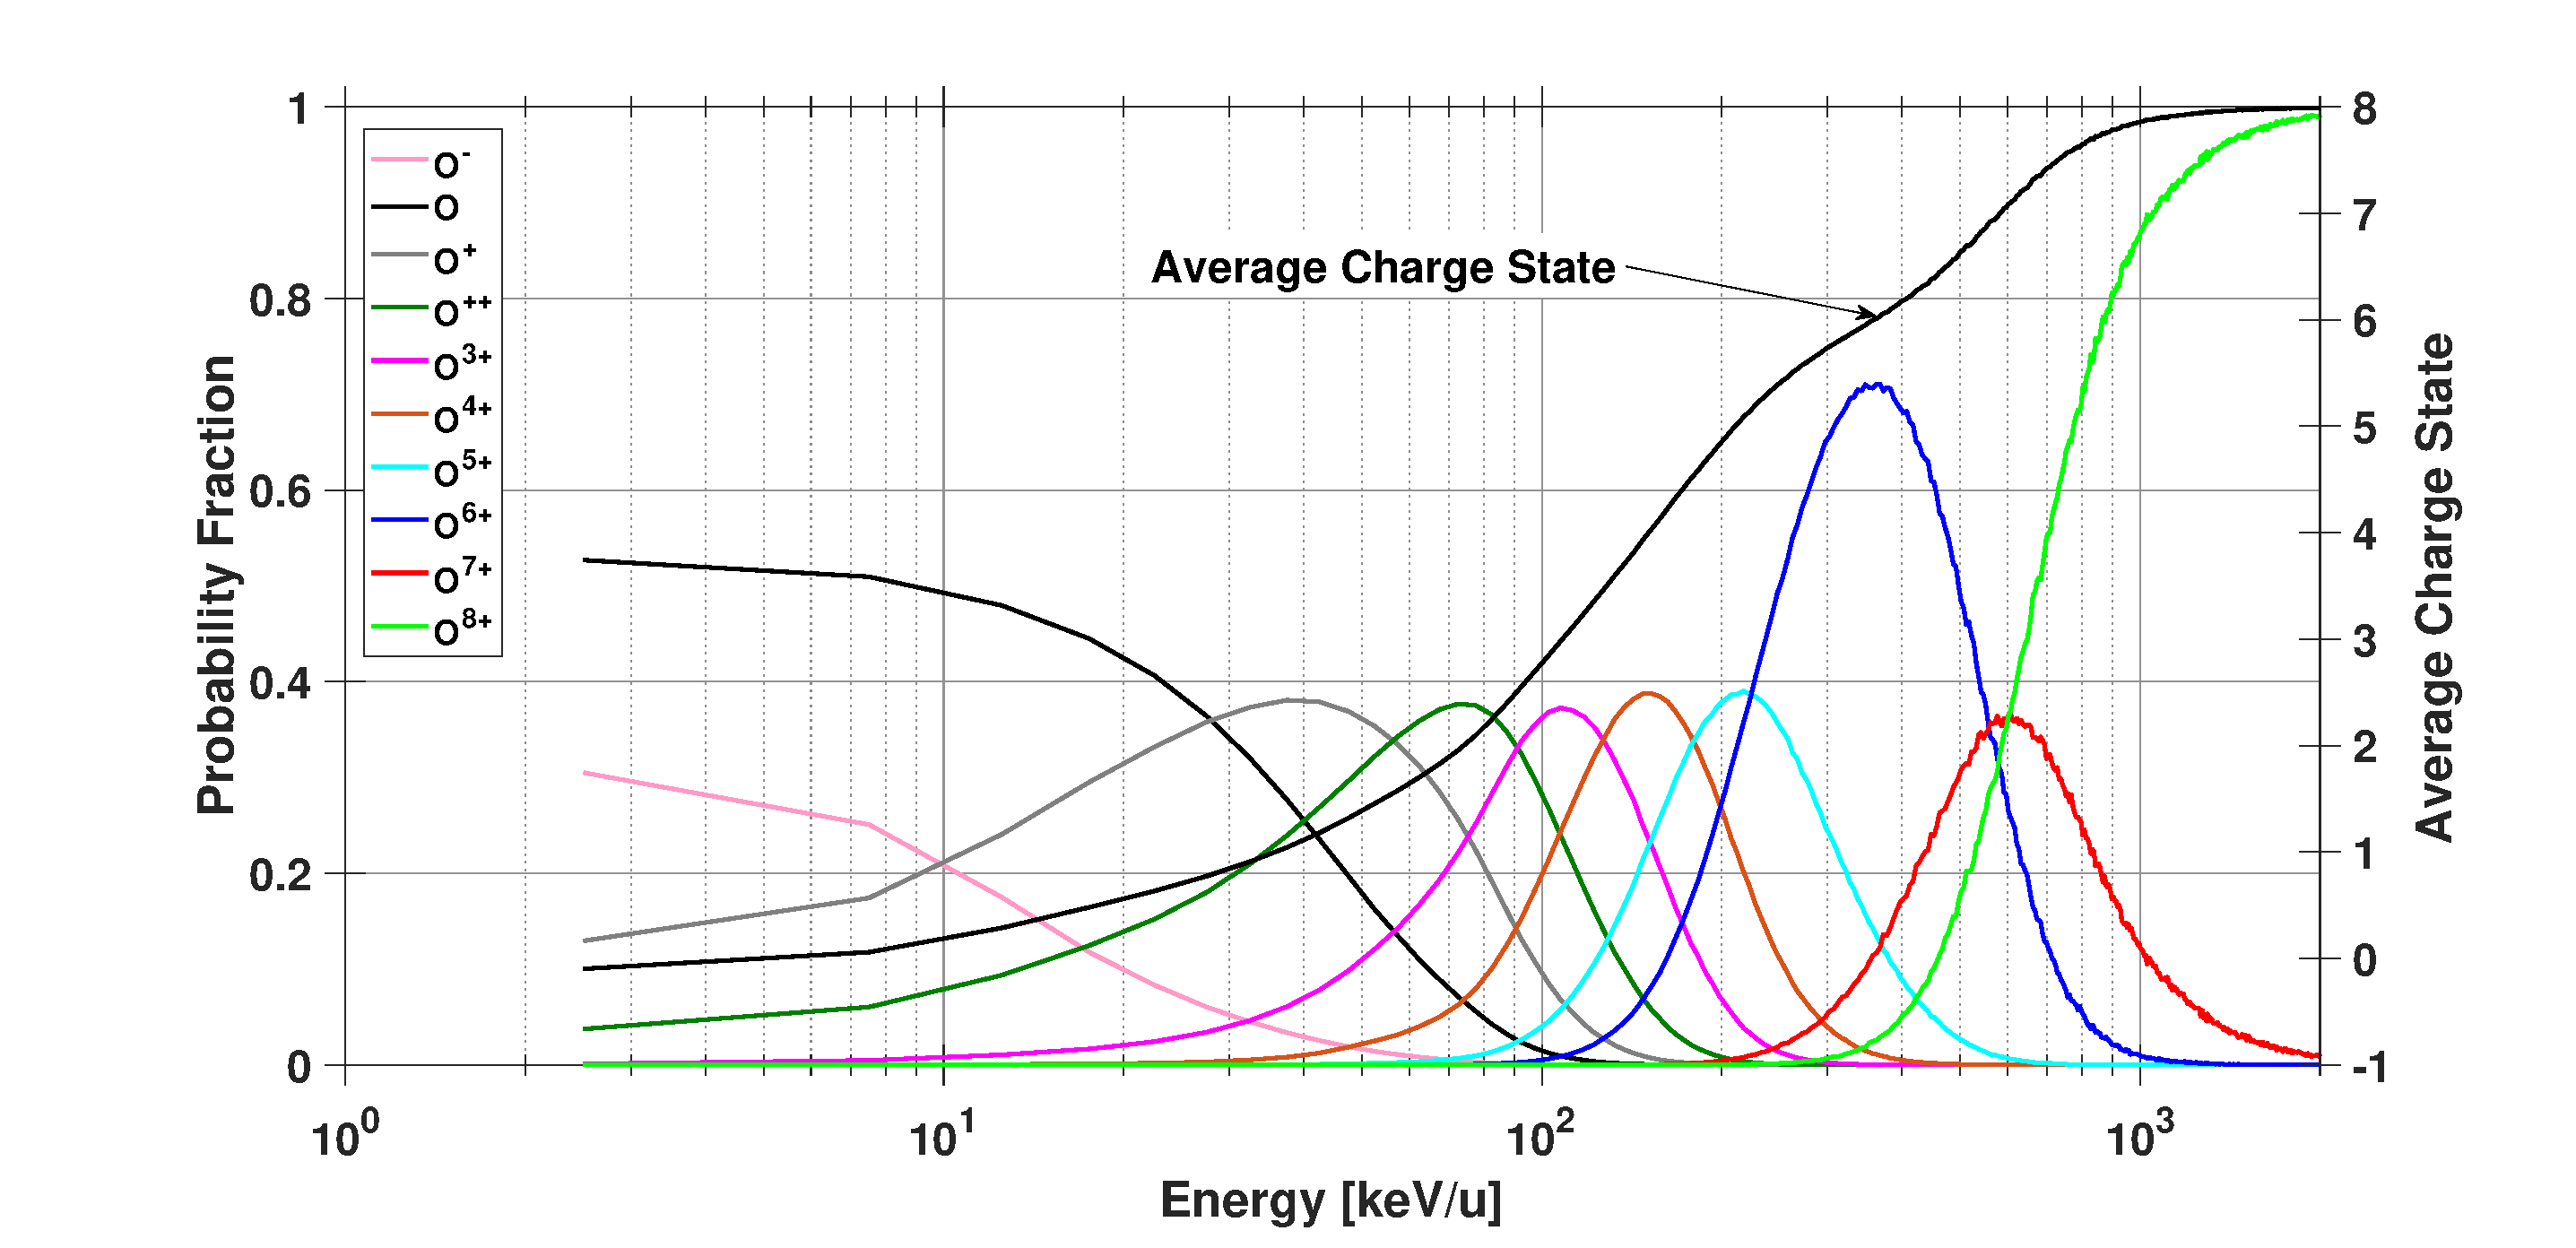
\includegraphics[width=\textwidth]{Figures/CSDoxy.eps}
    \caption{Oxygen charge state distribution}
    \label{fig:CSDoxy}
\end{figure}

\begin{figure}[ht]
    \centering
    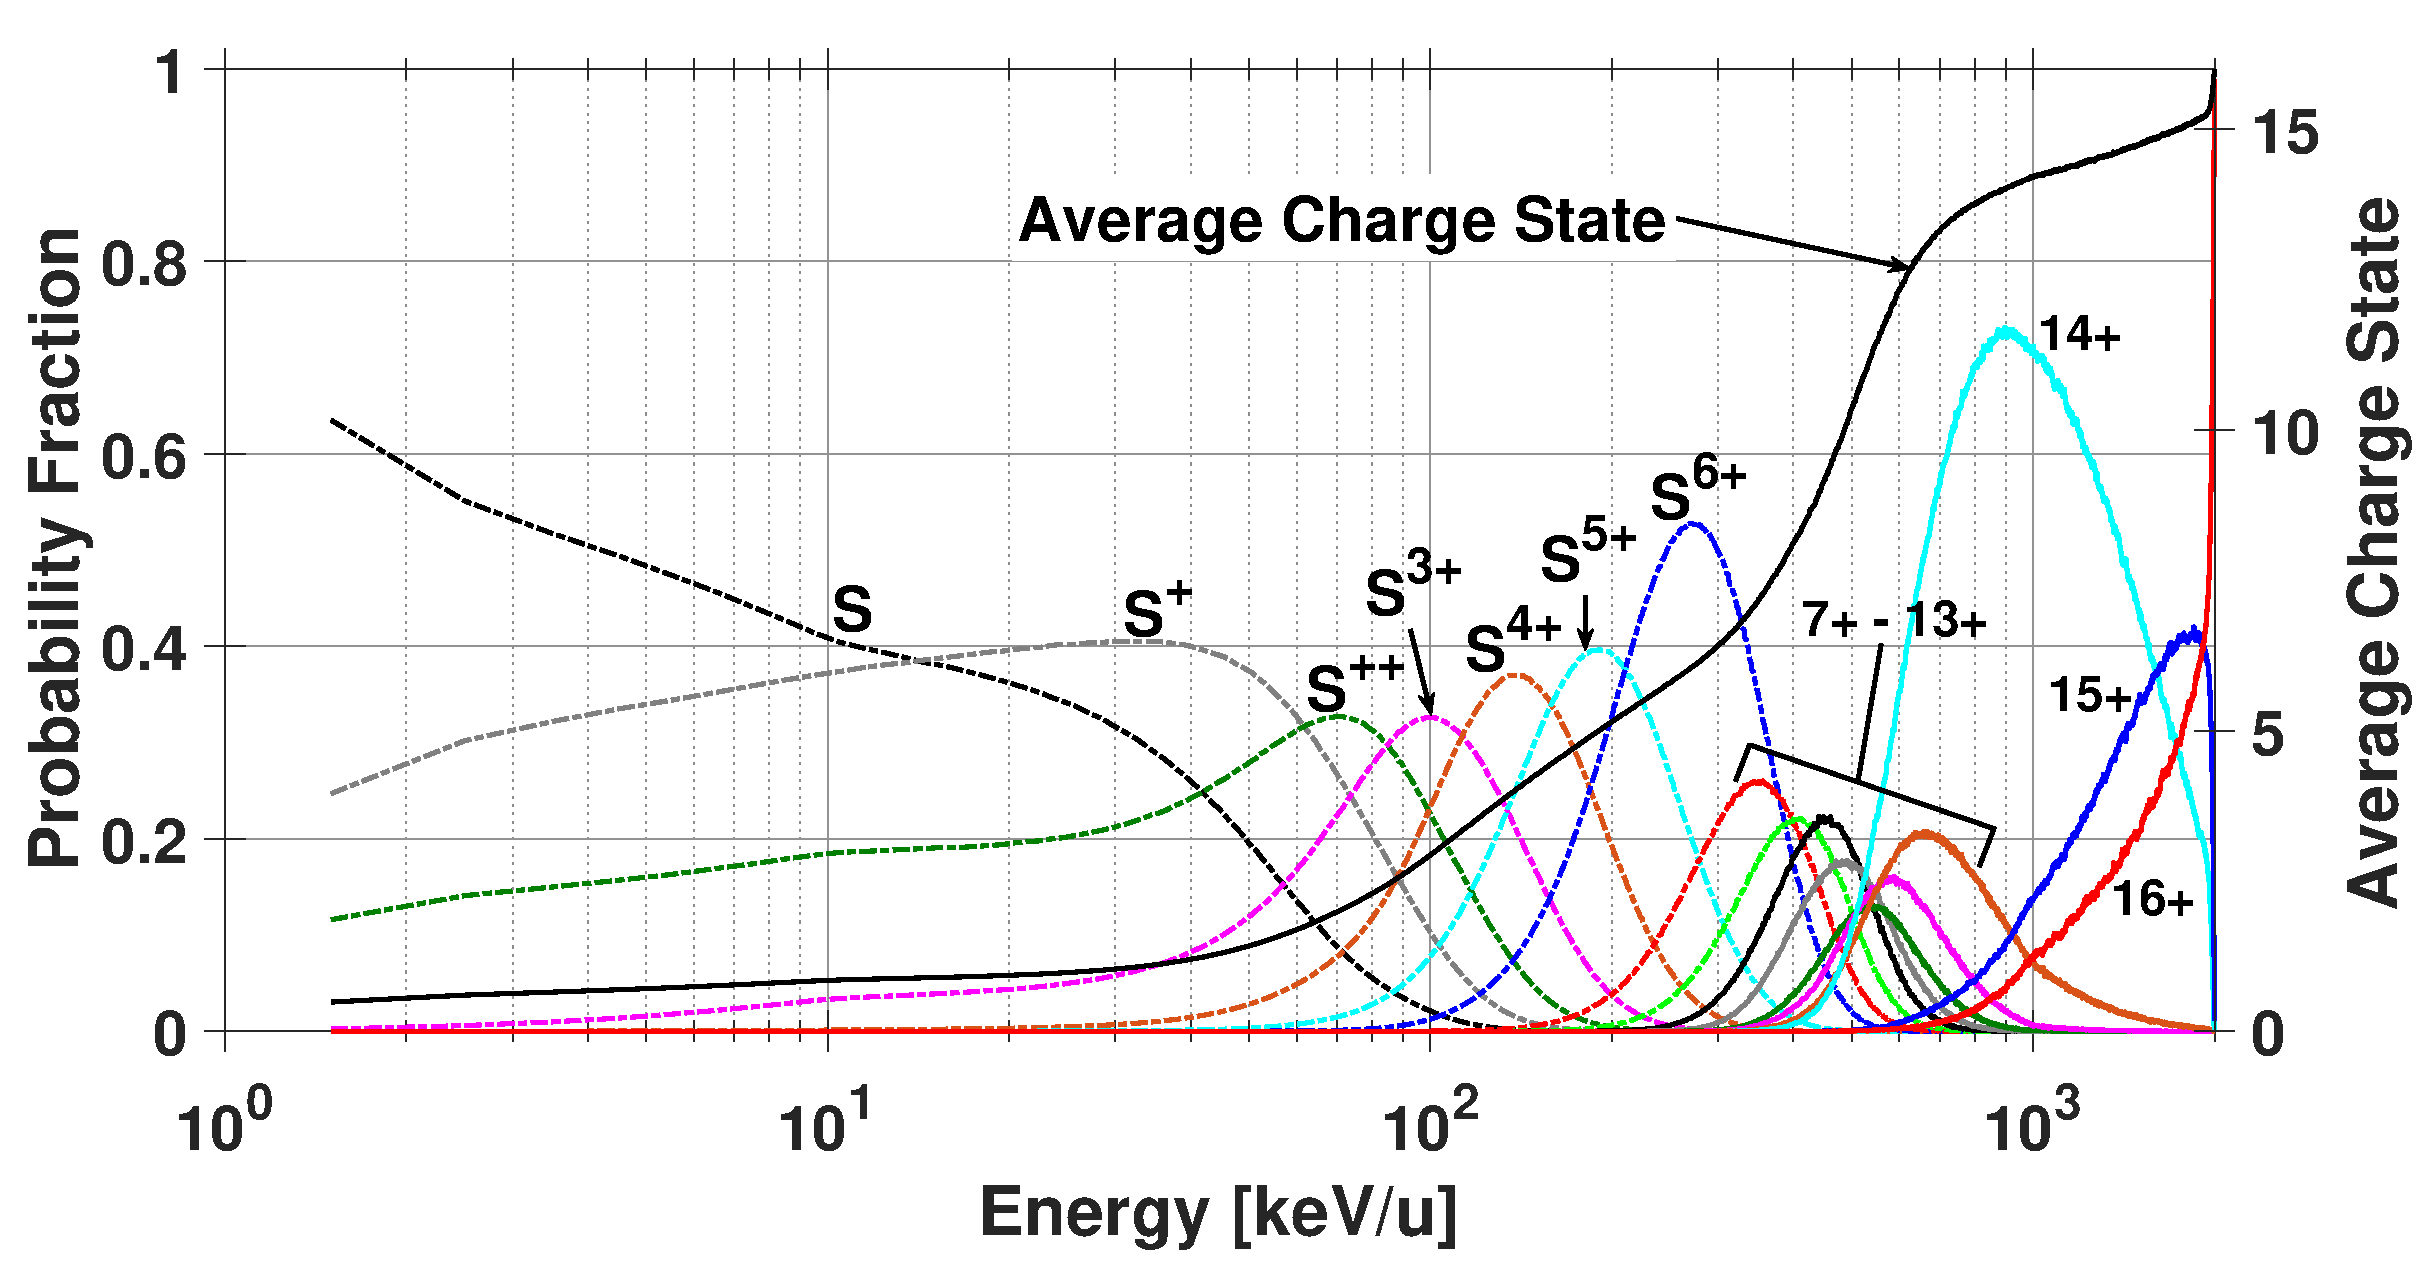
\includegraphics[width=\textwidth]{Figures/CSDsul.eps}
    \caption{Sulfur charge state distribution}
    \label{fig:CSDsul}
\end{figure}

The charge state equilibrium fractions demonstrate at what energy the ion will reach a given charge state regardless of the collision processes undergone or the initial ion energy; the ion history is immediately forgotten.
From here, one can see, at a glance, what energies are required for an ion to begin producing X-rays.
For both oxygen and sulfur the sixth charge state must be reached to begin producing X-rays (O$^{6+}$ and S$^{6+}$ with projectile excitation, or O$^{7+}$ and S$^{7+}$ with charge exchange).
These charge states are sufficiently reached for both species at an energy between 200-300 keV/u, where they become the most probable charge state for the given energy (a total energy of ~3.2 MeV and ~6.4 MeV for oxygen and sulfur, respectively).
These newly developed equilibrium fractions are no longer in agreement with previous models presented by \citet{ozak2010} and \citet{houston2018}, where they showed an O$^{6+}$ peak at nearly 1 MeV/u and an S$^{6+}$ peak at 600 keV/u.

Not only does it now require less energy to produce charge states capable of emitting X-rays, but the ions are not penetrating the atmosphere as deeply as was previously modeled because more energy is being lost in the middle energy range\footnote{See the stopping power discussion given by \citet{schultz2018}}, affecting the depth effects and predicted X-ray spectra.

\subsection{Depth Effects}

The opacity of the Jovian atmosphere is incorporated into the model using the optical depth of outgoing X-ray photons.
We look at three different path angles, 0$^{\circ}$, 80$^{\circ}$, and 90$^{\circ}$ (where the angle is measured with respect to the axis of rotation), and with two atmospheric profiles; the density profile shown in Figure \ref{fig:atm} and a well-mixed atmosphere as discussed in Section \ref{sec:atm}.
The optical depth is given by
\begin{equation}
    \tau(\lambda,z_{0})=Ch(\theta,z_{0})\sum_{j}\sigma_{j}^{abs}(\lambda)\int\displaylimits_{z_{0}}^{\infty}n_{j}(z)dz
    \label{eqn:tau}
\end{equation}
where $\tau(\lambda,z_{0})$ is the optical depth as a function of emitted photon wavelength, $\lambda$, and the altitude at which the emission occurred, $z_{0}$.
$Ch(\theta,z_{0})$ is the Chapman function, dependent upon the photon path angle, $\theta$, and the altitude.
$\sigma_j^{abs}(\lambda)$ is the absorption cross-section summed over each species, $j$ (H$_2$, He, and CH$_4$), and is a function of wavelength.
$n_j(z)$ is the neutral density of each atmospheric constituent as a function of altitude, integrated from the point of emission out through the top of the atmosphere.

The Chapman function has been approximated to $Ch(0^{\circ} \leq \theta \leq 80^{\circ},z_{0}) \approx \mathrm{sec}(\theta)$ for the first two exit angles and
\begin{equation}
    Ch(\frac{\pi}{2},z_{0})=\sqrt{\frac{R_J}{H(z_0)}\frac{\pi}{2}}
    \label{eqn:Chap}
\end{equation}
for $\theta$=90$^{0}$, where $R_J$ is the Jovian radii of 71,492 km and $H(z_0)$ is the scale height at altitude $z_0$.
The spectrum intensity, $I(\lambda)$ can then be calculated as
\begin{equation}
    4\pi I(\lambda)=\int\displaylimits_{z_0}^{\infty}P(\lambda,z)e^{-\tau(\lambda,z_0)}dz
    \label{eqn:I}
\end{equation}
where $P(\lambda,z)$ is the production rate of X-ray emission as a function of wavelength, $\lambda$ and altitude, $z$.
$P(\lambda,z)$ integrated over every value of $\lambda$ is equal to the ion production rate, $P(z)$, for a given charge state.
Therefore, to determine the production rate as a function of wavelength there are a couple of things to note before building synthetic spectra.

\subsection{Synthetic X-ray Spectra}
\label{sec:XraySpec}

An X-ray can be emitted through either the ion gaining an electron (what we refer to as charge transfer or charge exchange collisions) or the excitation of the ion (called direct excitation).
Both of these scenarios can result with an electron in an excited state where it will emit photons as it cascades down to a more energy favorable state.
Although we have many charge transfer and projectile excitation processes we only allow three of each type to ultimately result in the emission of a photon, TI, SC, and SC+SS for charge exchange and SI+SPEX, DI+SPEX, and TEX+SPEX for direct excitation.
Any collision that results in more than one electron being in an excited state at any time, whether it be through charge exchange, projectile excitation, or a combination of the two (e.g. DC or SC+SPEX collisions), we consider it much more likely for the Auger effect to take place than the emission of a photon.

\citet{hui2010} created synthetic, charge exchange, X-ray spectra for O$^{6+}$, O$^{7+}$, and S$^{6+}$-S$^{14+}$ that we have integrated into our model.
They were able to produce spectra vs. number of photons/ion which we have re-normalized for each charge state to total number of photons/charge state.
We then multiplied the production of each charge state, as a function of altitude, for the three charge exchange collisions that produce $P(\lambda,z)$.

Because charge transfer collisions are pulling an electron into the particle from outside of the ionization potential the electron will cascade from very high energy states until it has energetically relaxed.
This allows for high energy X-rays to be emitted and also many more cascading possibilities.
However, direct excitation excites an electron from the highest occupied electronic energy level, likely resulting in a change in principal quantum number of only one or two.
But once the electron is in a particular energy level it is unaware of whether it has been excited or picked up from outside of the ion; thus, at that point, the cascading probabilities should not differ between charge exchange or excitation.
It is important to note that electrons relaxing from charge transfer collisions will always be capable of following the same cascade path as an electron excited by direct excitation, but the reverse is not true.
This is due to direct excitation not starting with the electron at principal quantum number, $n=\infty$, and also forbidden excitation energy states.
Unfortunately, we do not have any state-selective excitation emission spectra of oxygen and sulfur; instead we need to apply an approximation to the charge exchange emission lines that represents the higher probability of starting at lower principal quantum numbers, rather than coming from principal quantum number, $n=\infty$, but have no approximation for the forbidden excitation transitions without a much more in-depth study of the matter.

We first approximate O$^{7+}$ as H, O$^{^6+}$ and S$^{14+}$ as He, S$^{13+}$ as Li, S$^{12+}$ as Li$^{+}$ or Be, S$^{11+}$ as Be$^{+}$, S$^{10+}$ as Be$^{++}$, and S$^{9+}$ as Be$^{3+}$, and assume the rest of the sulfur charge states will follow the same pattern shown by the higher charge states.
We then reviewed a number of articles concerning electron-impact excitation of lithium\citep{griffin2001}, beryllium\citep{bartschat1996}, lithium-like\citep{bely1966}, and beryllium-like\citep{bartschat1996} particles to understand the relative cross-sections between electronic energy levels.
The cross-sections for all of these cases were dominated by a change in principal quantum number of one, i.e. when an electron is excited it will typically ($\sim$80$\%$-85$\%$ of the time) only be excited to the next highest energy level.
Occasionally, $\sim$15$\%$ of the time, it will be excited to an even higher energy state.

Thus, we take the two or three most common emission lines, at lower photon energies, from the charge exchange synthetic spectra provided by \citet{hui2010} and distribute the direct excitation emission in the following way
\begin{equation}
    \sum_{i=1}^{2,3}\lambda_{i}f_{i}=E
    \label{eqn:DEemission}
\end{equation}
where $\lambda_{i}$ is the wavelength of the most likely emission line, or group of emission lines.
If there is a group of emission lines with similar wavelengths, the emission is distributed evenly among each wavelength because in this simple approximation we do not know the exact state-selective excitation transitions and forbidden excitation states have not been considered.
$f_{i}$ is the distribution of X-ray production given to each wavelength.
If only two lines, or groups of lines, are considered then $f_{1}$=0.85 and $f_{2}$=0.15; for three, $f_{1}$=0.80, $f_{2}$=0.15, and $f_{3}$=0.05.
$E$ is the total photon energy from emission.

To ensure this approximation is not violating conservation of energy, if $E>\Delta E$, where $\Delta E$ is the energy loss for SPEX at a given ion energy and charge state shown in \citet{schultz2018}, then the emission given in Equation \ref{eqn:DEemission} is re-normalized to conserve energy,
\begin{equation}
    \sum_{n=1}^{2,3}\lambda_{n}f_{n}\epsilon=E
\end{equation}
where $\epsilon=\Delta E/E$.
If $E<\Delta E$ then we assume the energy difference is due to emission from lower energy photons not considered in the X-ray spectrum and X-ray inefficiencies in emission from the way the electrons cascade through the electron orbitals.

To simulate a more realistic observation than perfect line emission that an X-ray observatory would detect, we apply a normalized Gaussian distribution to each data point to recover a new intensity:
\begin{equation}
    4\pi I'(\lambda)=\sum_{\lambda_{\mu}}\frac{1}{\sqrt{2\pi\sigma^2}}I(\lambda)e^{-\frac{(\lambda-\lambda_{\mu})^2}{2\sigma^2}}
\end{equation}
where $\lambda$ is now the full spectrum (in eV) which we allow to go from 100 eV to 3500 eV. $\lambda_{\mu}$ is the original wavelength data points, $\sigma^2$ is the variance which we have set to 20 eV.

\subsection{Juno Data}

Maybe send to Abi and/or Dennis??

\section{Results}

\subsection{Ion Production Rates}

When referring to ion production rates, it is important to note that we are only referencing production from charge transfer collisions, i.e. $X^q \rightarrow X^{q-1}$, because that is what produces photon emission.
Therefore, the ion production rate as a function of altitude, $P(z)$, can be calculated outright for a product ion species, $i$, (e.g. O$^{7+}$ or S$^{8+}$) as follows:
\begin{equation}
    P(z)=\int\displaylimits_{z_0}^{\infty}n(z)[\sigma_{q,q-1}^i(E(z))]\phi_q^i\Phi^idz
\end{equation}
where $n(z)$ is the neutral atmosphere density of H$_2$, $\sigma_{q,q-1}^i(E(z))$ denotes the charge transfer cross-sections for species $i$ with energy $E$ at altitude $z$, $\phi_q^i$ is the equilibrium fraction given in Equations \ref{eqn:EqProb} and \ref{eqn:EqProbNorm}, and $\Phi^i$ represents the total flux of the initial ion beam.
However, our model uses a Monte Carlo method that tracks each ion individually and counts each charge exchange collision that occurs for a given charge state.
These collisions are tracked through a set of altitude bins with a given input of $\sim$20,000 incident ions and then the production rate is normalized to an input of 1 ion/cm$^2$/s.
The production rates for O$^{6+}$ and O$^{7+}$ are shown in Figures \ref{fig:O6+Prod} and \ref{fig:O7+Prod}.
It is to be emphasized, these production rates only include charge exchange from the three collisions discussed in Section \ref{sec:XraySpec}, that is TI, SC, and SC+SS; although other processes can contribute to lowering the overall charge state without emitting a photon (e.g. the Auger process).

\begin{figure}[ht]
    \centering
    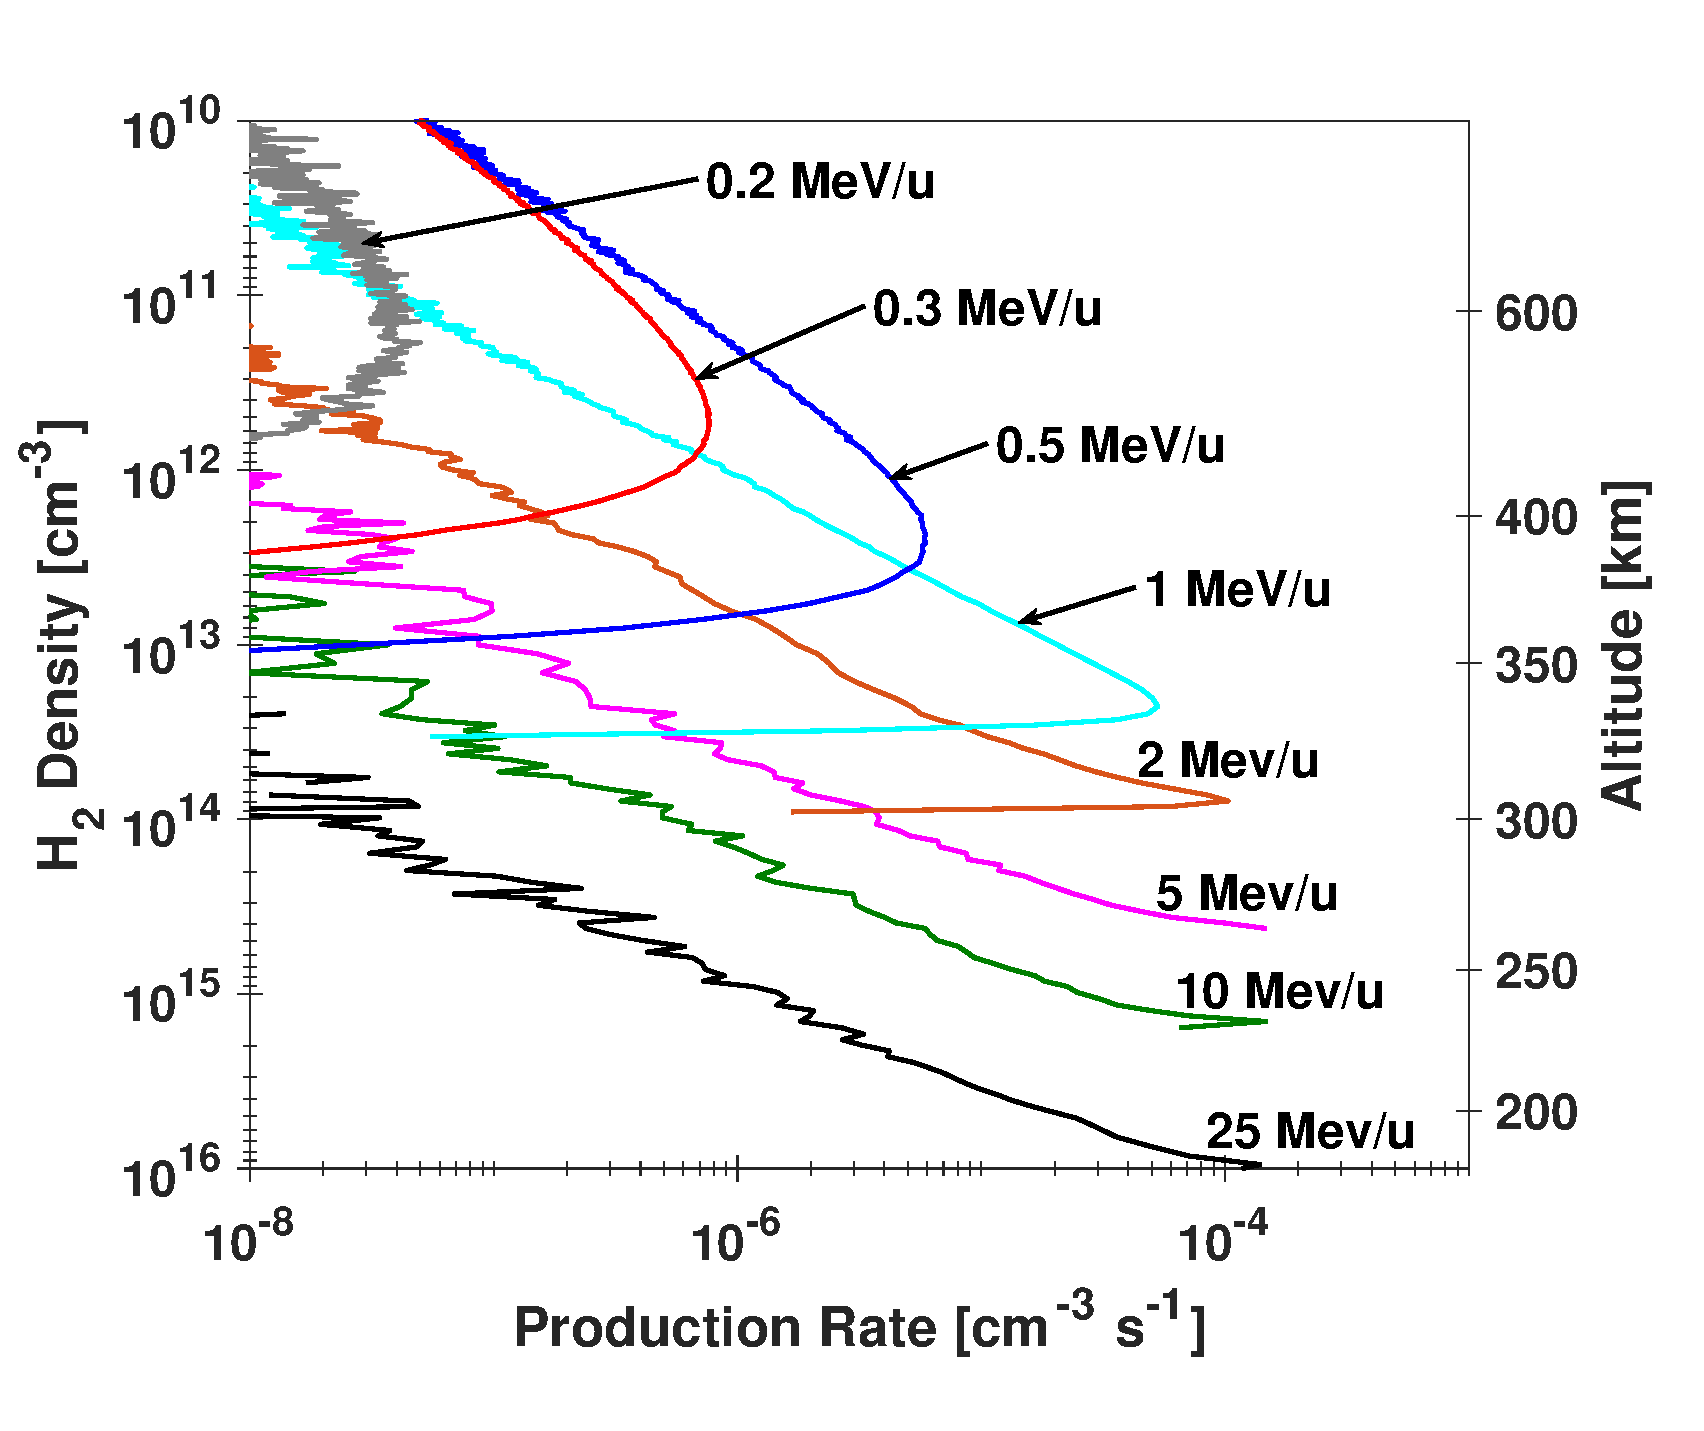
\includegraphics[width=\textwidth]{Figures/O6CXProd.eps}
    \caption{The O$^{6+}$ production rate from TI, SC, and SC+SS vs. H$_2$ density [cm$^{-3}$] and altitude [km] for various incident ion energies (E=0.2, 0.3, 0.5, 1.0, 2.0, 5.0, 10.0, and 25.0 MeV/u).}
    \label{fig:CSDoxy}
\end{figure}

\begin{figure}[ht]
    \centering
    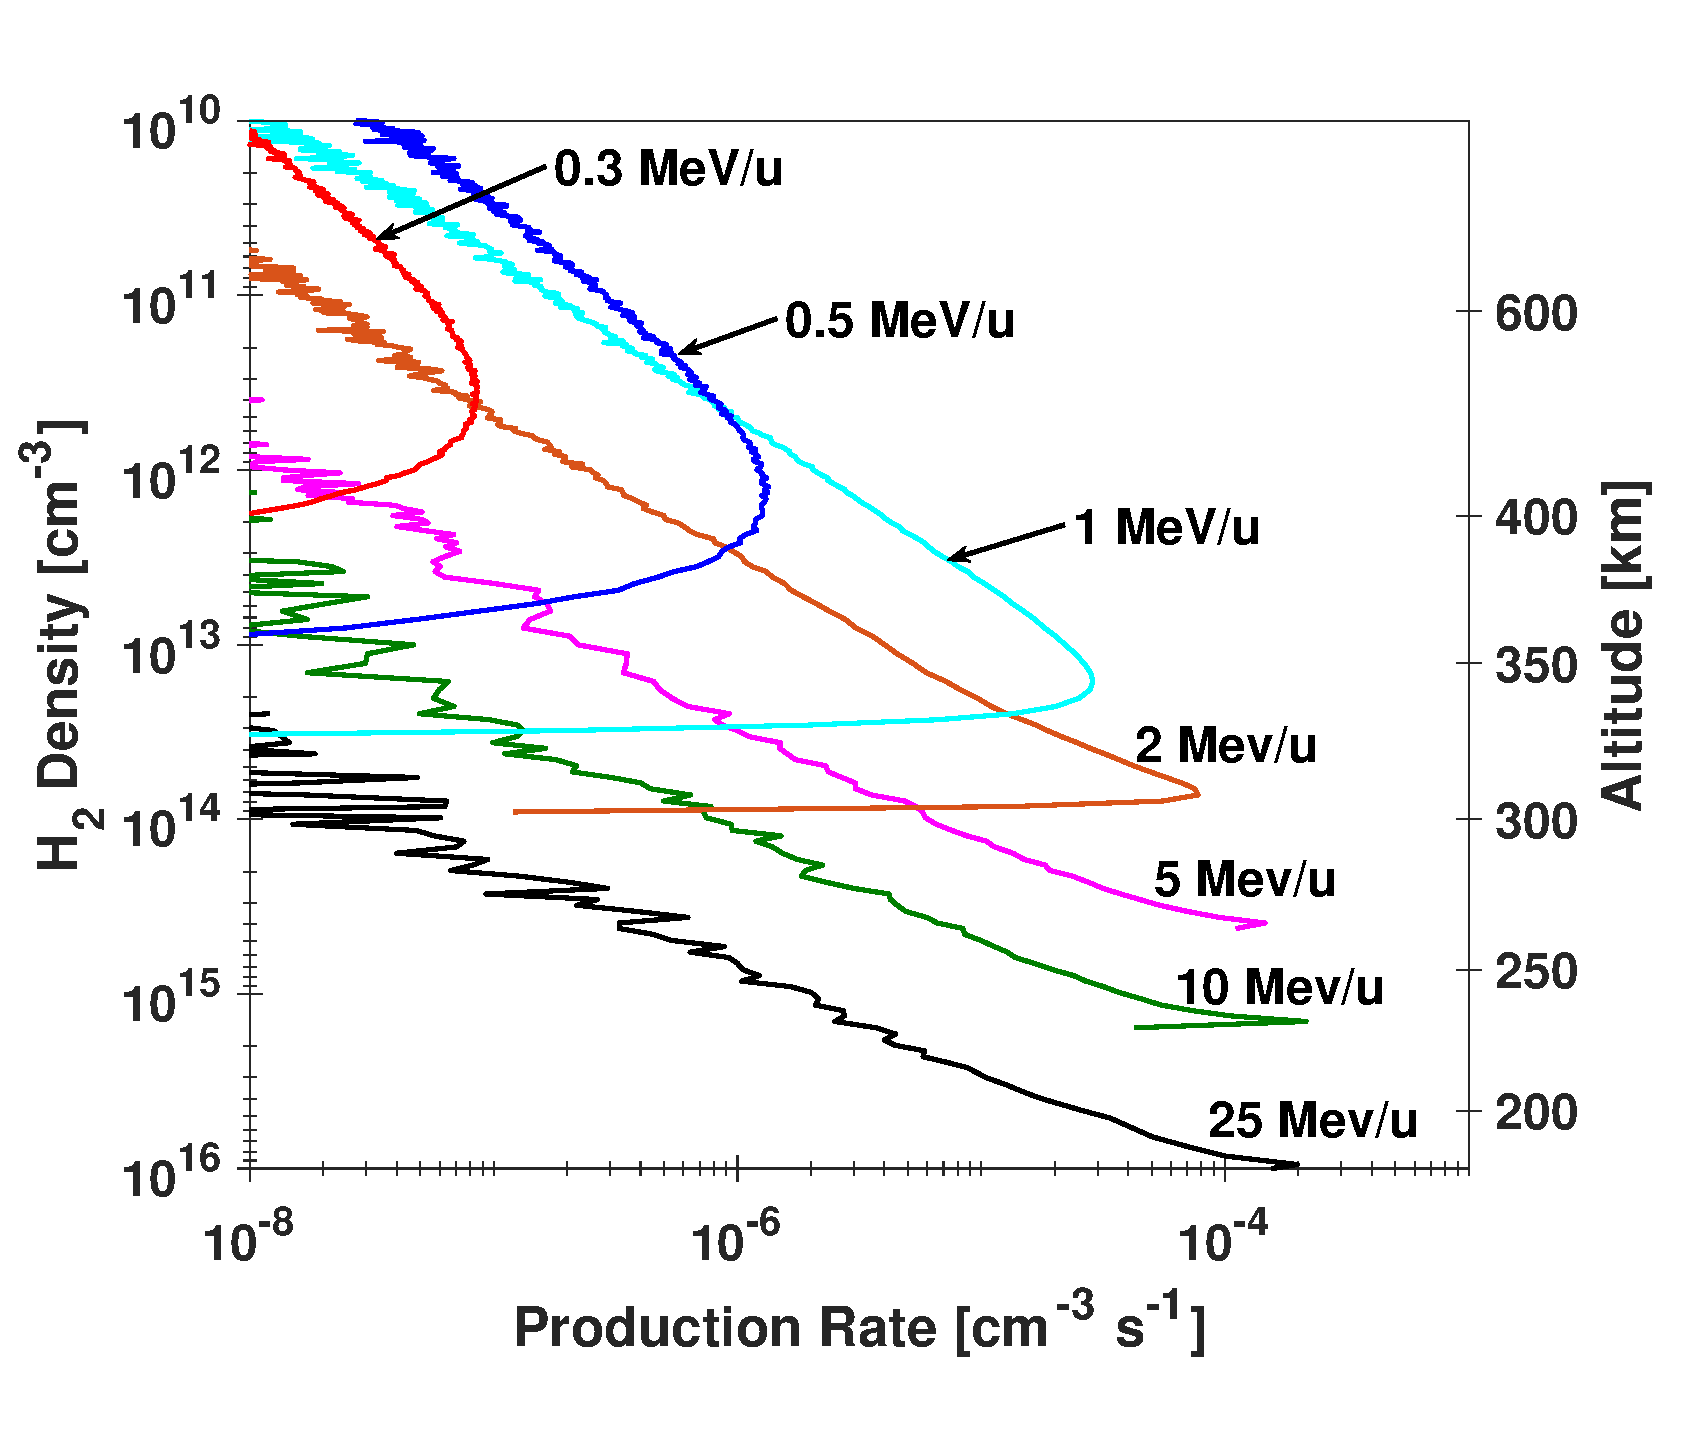
\includegraphics[width=\textwidth]{Figures/O7CXProd.eps}
    \caption{The O$^{7+}$ production rate from TI, SC, and SC+SS vs. H$_2$ density [cm$^{-3}$] and altitude [km] for various incident ion energies (E=0.3, 0.5, 1.0, 2.0, 5.0, 10.0, and 25.0 MeV/u).}
    \label{fig:CSDsul}
\end{figure}

%%%%%%%%%%%%%%%%%%%%%%%%%%%%%%%%%%%%%%%%%%%%%%%%%%%%%%%%%%%%%%%%
%
%  ACKNOWLEDGMENTS
%
% The acknowledgments must list:
%
% >>>>	A statement that indicates to the reader where the data
% 	supporting the conclusions can be obtained (for example, in the
% 	references, tables, supporting information, and other databases).
%
% 	All funding sources related to this work from all authors
%
% 	Any real or perceived financial conflicts of interests for any
%	author
%
% 	Other affiliations for any author that may be perceived as
% 	having a conflict of interest with respect to the results of this
% 	paper.
%
%
% It is also the appropriate place to thank colleagues and other contributors.
% AGU does not normally allow dedications.


\acknowledgments
Enter acknowledgments, including your data availability statement, here.


%% ------------------------------------------------------------------------ %%
%% References and Citations

\bibliography{Biblio/mybiblio}


\end{document}
